\documentclass[xetex,table]{beamer}

\usepackage{fontspec}
\usepackage[autostyle]{csquotes}
\usepackage{hyperref}
\usepackage{color}
\usepackage{setspace}
\usepackage{listings}
\usepackage{minted}

\usetheme{Pittsburgh}
\usecolortheme{beaver}

\title{Programmazione a oggetti in C nel kernel di Linux}
\author{Luca Ceresoli}
\date{}

\AtBeginSection[]
{
  \begin{frame}{}
    \huge
    \begin{center}
      \insertsection
    \end{center}
  \end{frame}
}

\begin{document}

\maketitle

\section{Introduzione}

\begin{frame}
  \frametitle{Programmazione non orientata agli oggetti}
  \begin{itemize}
  \item Il software è un insieme di procedure che manipolano dati
  \item Le procedure accedono ai dati direttamente
  \end{itemize}
\end{frame}

\begin{frame}[fragile]
  \frametitle{Esempio: shopping cart}
  \begin{minted}[fontsize=\scriptsize]{c++}
    struct Item {
      string name;
      int    price;
    };

    int main() {
      list<Item> cart1, cart2;
      Item kr = {"The C Programming Language", 53};
      Item bs = {"The C++ Programming Language", 56};
      Item bc = {"Understanding the Linux Kernel", 45};
      cart1.push_back(kr);
      cart1.push_back(bs);
      cart2.push_back(kr);
      cart2.push_back(bc);
      int total1 = 0, total2 = 0;
      for (Item &i: cart1)
        total1 += i.price;
      for (Item &i: cart2)
        total2 += i.price;
      cout << "Cart1 total: " << total1 << endl;
      cout << "Cart2 total: " << total2 << endl;
    }
  \end{minted}
\end{frame}

\begin{frame}
  \frametitle{Programmazione orientata agli oggetti}
  \begin{itemize}
  \item Ogni entità logica è rappresentata da un oggetto
  \item Un oggetto contiene:
    \begin{itemize}
    \item {\em proprietà}: i dati che la definiscono
    \item {\em metodi}: possibili azioni che agiscono sui dati
  \end{itemize}
  \item Classe:
    \begin{itemize}
    \item descrizione astratta di oggetti dello stesso tipo
    \end{itemize}
  \end{itemize}
\end{frame}

\begin{frame}[fragile]
  \frametitle{Esempio ad oggetti /1}
  \begin{minted}[fontsize=\scriptsize]{c++}
    struct Item {
      string name;
      int    price;
    };

    class ShoppingCart {
      public:
        void   add(Item &item);
        int    getTotal();
      private:
        list<Item> items;
    };

    void ShoppingCart::add(Item &item) {
      items.push_back(item);
    }

    int ShoppingCart::getTotal() {
      int total = 0;
      for (Item &i: items)
        total += i.price;
      return total;
    }
  \end{minted}
\end{frame}

\begin{frame}[fragile]
  \frametitle{Esempio ad oggetti /2}
  \begin{minted}[fontsize=\scriptsize]{c++}
    int main()
    {
      ShoppingCart cart1, cart2;
      Item kr = {"The C Programming Language", 53};
      Item bs = {"The C++ Programming Language", 56};
      Item bc = {"Understanding the Linux Kernel", 45};
      cart1.add(kr);
      cart1.add(bs);
      cart2.add(kr);
      cart2.add(bc);
      cout << "Cart1 total: " << cart1.getTotal() << endl;
      cout << "Cart2 total: " << cart2.getTotal() << endl;
    }
  \end{minted}
\end{frame}

\begin{frame}
  \frametitle{Linguaggio C}
  \begin{itemize}
  \item Un linguaggio a oggetti (C++) offre molti vantaggi
  \item Ma molti software sono tuttora scritti in C
    \begin{itemize}
    \item Software semplici
      \begin{itemize}
      \item Firmware per microcontrollori
      \item Utility di dimensioni contenute
      \end{itemize}
    \item Ma anche software molto complessi (e strutturati a oggetti)
      \begin{itemize}
      \item Linux kernel
      \item GTK+
      \item EFL
      \end{itemize}
    \end{itemize}
  \end{itemize}
\end{frame}

\section{Classi e oggetti in C}

\begin{frame}
  \frametitle{Classi e oggetti in C}
  \begin{itemize}
  \item In C si possono creare delle ``classi'' usando le \texttt{struct}
    \begin{itemize}
    \item Contengono le proprietà (dati), non i metodi
    \item Per ricreare i metodi usiamo normali funzioni
      \begin{itemize}
      \item Che come primo parametro ricevono un puntatore alla struct
      \end{itemize}
    \end{itemize}
    \item Proprietà e metodi non sono legati dal linguaggio, ma da una
      convenzione
  \end{itemize}
\end{frame}

\begin{frame}[fragile]
  \frametitle{Esempio ad oggetti in C}
  \begin{minted}[fontsize=\scriptsize]{c}
    struct ShoppingCart {
      Item items[100];
    };

    int main()
    {
      ShoppingCart cart1, cart2;
      shoppingcart_initialize(&cart1);
      shoppingcart_initialize(&cart2);
      Item kr = {"The C Programming Language", 53};
      Item bs = {"The C++ Programming Language", 56};
      Item bc = {"Understanding the Linux Kernel", 45};
      shoppingcart_add(&cart1, &kr);
      shoppingcart_add(&cart1, &bs);
      shoppingcart_add(&cart2, &kr);
      shoppingcart_add(&cart2, &bc);
      cout << "Cart1 total: " << shoppingcart_get_total(&cart1) << endl;
      cout << "Cart2 total: " << shoppingcart_get_total(&cart2) << endl;
    }
  \end{minted}
\end{frame}

\section{Ereditarietà e polimorfismo}

\begin{frame}
  \frametitle{Ereditarietà}
  \begin{itemize}
  \item Da una classe base, se ne crea un'altra (sottoclasse)
    \begin{itemize}
    \item che ne eredità proprietà e metodi
    \item e ne aggiunge di nuovi
    \item o modifica il comportamento di quelli esistenti
    \end{itemize}
  \item Si crea una gerarchia di classi
  \end{itemize}
  \begin{center}
    \includegraphics[height=0.6\textheight]{images/inheritance.pdf}
  \end{center}
\end{frame}

\begin{frame}
  \frametitle{Polimorfismo}
  \begin{itemize}
  \item Lo stesso metodo può agire su oggetti di classi diverse
  \item Ogni sottoclasse può aumentare o sostituire il metodo della
    classe base
  \item Esempio: \texttt{Shape::draw()} può essere chiamato su oggetti
    \texttt{Rectangle} o \texttt{Circle}
  \end{itemize}
\end{frame}

\section{Il kernel di Linux}

\begin{frame}
  \frametitle{Il kernel}
  \begin{itemize}
  \item È il ``nocciolo'' del sistema operativo
  \item Gestisce tutte le risorse hardware, i processi, la memoria e
    molto altro
  \item Scritto in C
  \item Fortemente strutturato ad oggetti
    \begin{itemize}
    \item Il {\em device model}: struttura dei device e dei device drivers
    \item Il {\em Virtual Filesystem}: gestione uniforme di diversi filesystem
    \item \dots
    \end{itemize}
  \end{itemize}
\end{frame}

\begin{frame}
  \frametitle{Il device model}
  \begin{itemize}
  \item Modello a oggetti di tutte le periferiche del computer
  \item Introdotto in Linux 2.6 (2003)
  \item Permette:
    \begin{itemize}
    \item Power management
    \item Visibilità all'utente delle periferiche connesse
      \begin{itemize}
      \item \texttt{sysfs}
      \item \texttt{lshw}
      \end{itemize}
    \item Hotplug
    \item Object lifecycle
    \end{itemize}
  \end{itemize}
\end{frame}

\begin{frame}
  \frametitle{Il device model --- class diagram}
  \begin{center}
    \includegraphics[height=0.6\textheight]{images/device-model.pdf}
  \end{center}
\end{frame}

\begin{frame}
  \frametitle{\texttt{struct kobject}}
  \begin{itemize}
  \item Classe base da cui derivano le altre
    \begin{itemize}
    \item Collegamenti tra oggetti
      \begin{itemize}
      \item Esempio: un device USB punta all'hub USB cui è connesso
      \end{itemize}
    \item Rappresentazione in sysfs
      \begin{itemize}
      \item Attributi del kobject diventano file in \texttt{/sys}
      \item Collegamenti (puntatori) tra kobject diventano link in
        \texttt{/sys}
      \end{itemize}
    \item Generazione eventi hotplug
    \item Reference counting
    \end{itemize}
  \end{itemize}
\end{frame}

\section{Ereditarietà dei dati}

\begin{frame}[fragile]
  \frametitle{Ereditarierà dei dati in C++}
  \begin{minted}[fontsize=\scriptsize]{c++}
    class Shape
    {
     private:
      float x, y;
    }

    class Circle : public Shape
    {
     public:
      float left() {
        return (x - radius);
      }
      float right() {
        return (x + radius);
      }
     private:
      float radius;
    }
  \end{minted}
\end{frame}

\begin{frame}[fragile]
  \frametitle{Ereditarierà dei dati in C nel kernel}
  \begin{itemize}
  \item Realizzata con diverse tecniche
    \begin{itemize}
    \item Embedded structures (il più utilizzato)
    \item Unions
    \item Void pointers
    \end{itemize}
  \end{itemize}
\end{frame}

\begin{frame}[fragile]
  \frametitle{Embedded structures /1}
  \texttt{struct kobject}

  \begin{minted}[fontsize=\scriptsize]{c}
    struct kobject {
      const char          *name;

      struct kobject      *parent;
      struct kernfs_node  *sd; /* sysfs directory entry */

      struct kref          kref;

      /* ... */
    };
  \end{minted}
  {\tiny Source:
    \url{http://lxr.free-electrons.com/source/include/linux/kobject.h?v=4.8#L63}}
\end{frame}

\begin{frame}[fragile]
  \frametitle{Embedded structures /2}
  \texttt{struct device} eredita da \texttt{struct kobject}

  \begin{minted}[fontsize=\scriptsize]{c}
    struct device {
      struct kobject        kobj;

      struct dev_pm_info    power;
      struct dev_pm_domain *pm_domain;

      dev_t                 devt;    /* dev_t, creates the sysfs "dev" */

      /* ... */
    };
  \end{minted}
  {\tiny Source:
    \url{http://lxr.free-electrons.com/source/include/linux/device.h?v=4.8#L780}}
\end{frame}

\begin{frame}[fragile]
  \frametitle{Embedded structures /3}
  \texttt{struct input\_dev} eredita da \texttt{struct device}

  \begin{minted}[fontsize=\scriptsize]{c}
    struct input_dev {
      const char *name;

      unsigned long evbit[BITS_TO_LONGS(EV_CNT)];
      unsigned long keybit[BITS_TO_LONGS(KEY_CNT)];

      struct device dev;

      /* ... */
    };
  \end{minted}
  {\tiny Source:
    \url{http://lxr.free-electrons.com/source/include/linux/input.h?v=4.8#L121}}
\end{frame}

\begin{frame}[fragile]
  \frametitle{Accesso ai dati}
  \begin{itemize}
  \item Dalla classe derivata alla classe base:
    \begin{minted}[fontsize=\scriptsize]{c}
      my_input_device.dev.power
      my_input_device.dev.kobj.name
    \end{minted}
  \item Dalla classe base alla classe derivata:
    \begin{itemize}
    \item \mint{c}|container_of()|
    \end{itemize}
  \end{itemize}
\end{frame}

\begin{frame}[fragile]
  \frametitle{La macro \texttt{container\_of()}}
    \begin{itemize}
    \item \mint{c}|container_of(ptr, type, member)|
      {\tiny\url{http://lxr.free-electrons.com/source/include/linux/kernel.h?v=4.8#L830}}
    \item Esempio: \texttt{to\_input\_dev()} dato un puntatore a
      \texttt{struct device} restituisce un puntatore alla
      \texttt{struct input\_device} che lo contiene
    \end{itemize}
  \begin{minted}[fontsize=\scriptsize]{c}
    struct input_dev {
      unsigned long evbit[BITS_TO_LONGS(EV_CNT)];
      unsigned long keybit[BITS_TO_LONGS(KEY_CNT)];

      struct device dev;

      /* .. */
    };
    #define to_input_dev(d) container_of(d, struct input_dev, dev)
  \end{minted}
  {\tiny Source:
    \url{http://lxr.free-electrons.com/source/include/linux/input.h?v=4.8#L121}}
\end{frame}

\begin{frame}
  \frametitle{Grazie per l'attenzione!}

  \begin{center}
    {\Huge Domande?}

    \vspace{0.1\textheight}

    \href{mailto:luca@lucaceresoli.net}{luca@lucaceresoli.net}\\
    \url{http://lucaceresoli.net}

    \textcopyright{} Copyright 2016, Luca Ceresoli\\

    \vspace{0.2\textheight}

    \tiny
    Materiale rilasciato sotto licenza\\
    Creative Commons Attribution - Share Alike 3.0 \\
    \url{https://creativecommons.org/licenses/by-sa/3.0/} \\
\end{center}
\end{frame}

\end{document}
